\section{Durchführung}
\label{sec:Durchführung}

In Abbildung \ref{fig:Aufbau_Durchfuehrung} ist die gesamte Messapparatur ersichtlich. 
Eine Lichtquelle, im Folgenden ein Laser mit vorteilhaft großer Kohärenzlänge, trifft auf den Strahlteiler; die beiden Strahlen werden an Spiegeln jeweils 
reflektiert und von einem Photoelement aufgefangen, welches die Impulse an ein Zählwerk weiterleitet. 
Im einem der beiden Strahlengang befindet sich die Ausgleichsplatte, sowie lässt sich einer der beiden Spiegel mittels 
dahinter befestigter Rändelschrauben minimal justieren, um anfangs die Lichtzentren beider Teilstrahlen auf einen Punkt am Photoelement 
zu lenken. 
An dem anderen Spiegel befindet sich die Mikrometerschraube, die den anderen Spiegel ausschließlich vor- und rückwärts bewegt. 
Dies bewirkt einen optischen Wegunterschied durch die geometrische Veränderung der Weglängendifferenz. 
Da die Apparatur sehr präzise Justierungen benötigt, wird diese über einen Synchronmotor verstellt, der durch einfaches Bedienen 
der Schaltknöpfe in Gang gesetzt werden kann. 
Die Übersetzung von der Anzeige der Weglänge beträgt $1:5.017$.
In der Messzelle der Länge $b=\SI{50}{\milli\meter}$ kann mithilfe einer Vakuumpumpe eine Druckdifferenz zur Umgebungsluft hergestellt werden, 
um entsprechend den Brechindex der Umgebungsluft zu bestimmen.

\begin{figure}
    \centering
    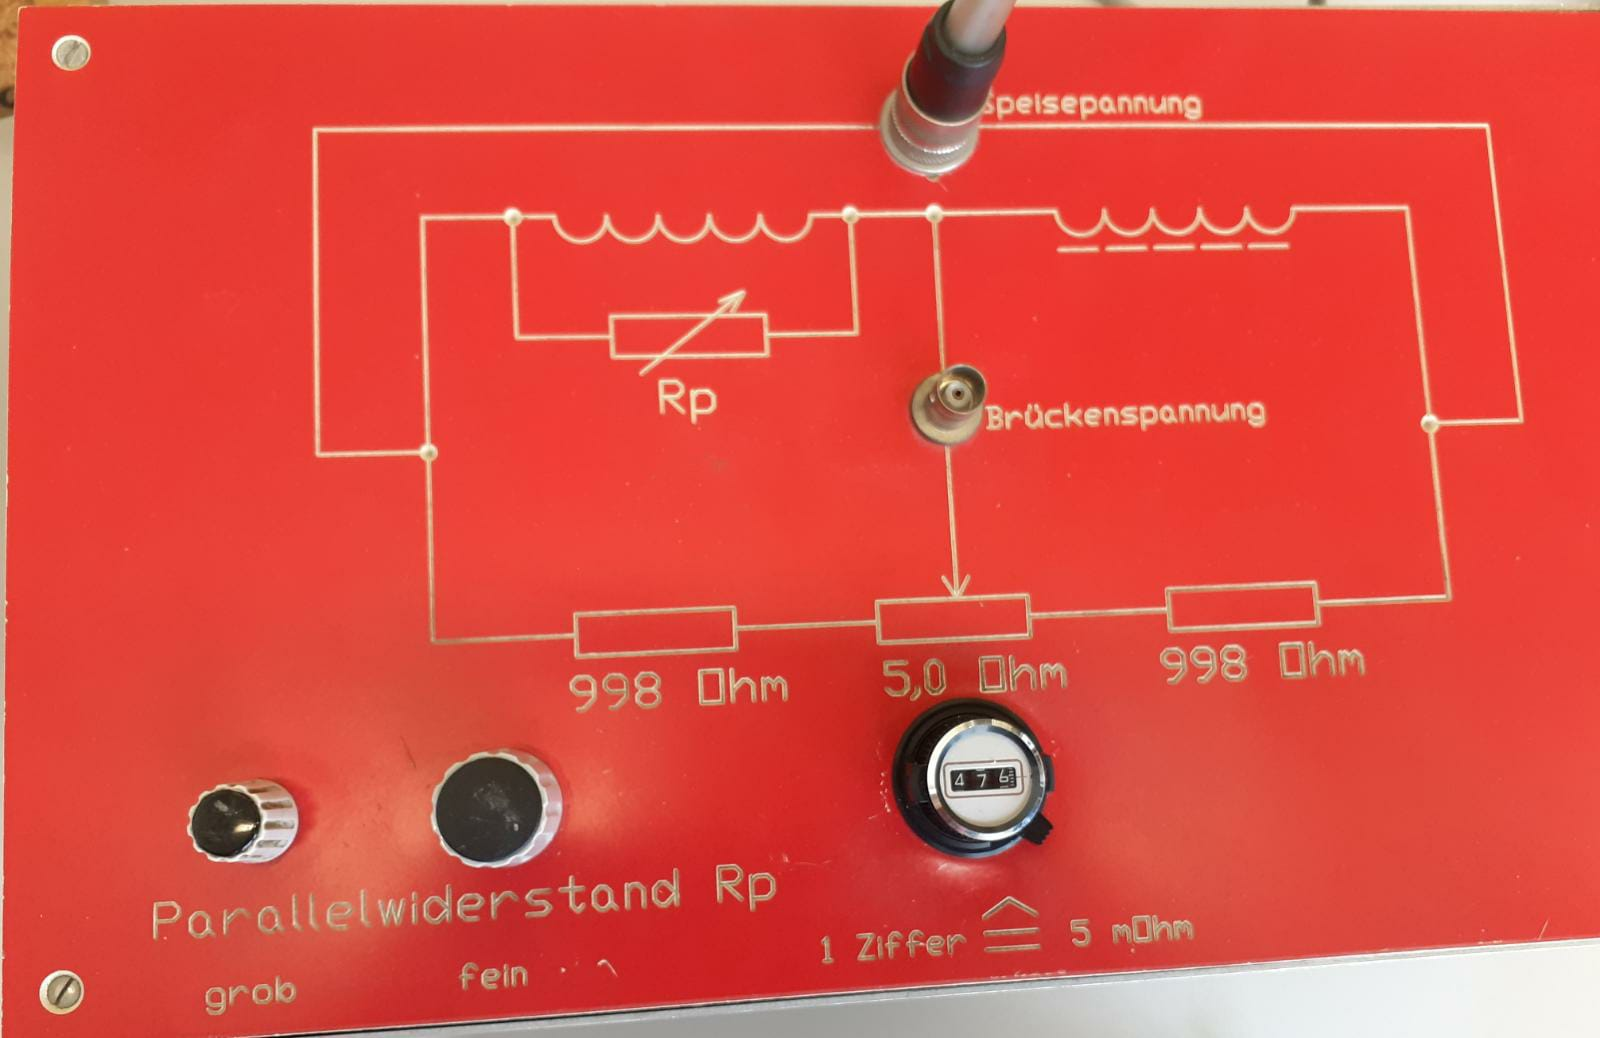
\includegraphics[width=\textwidth]{plots/Durchführung.png}
    \caption{Der gesamte Aufbau bei der Verwendung des Interferometers.}
    \label{fig:Aufbau_Durchfuehrung}
\end{figure}

Nach der beschriebenen Justierung durch die Rändelschrauben wird die Anzahl der Interferenzstreifen mittels des Zählwerks 
gemessen, während zeitgleich der Synchronmotor die Mikrometerschrauben bedient. 
Die Weglängendifferenz muss zusammen mit der Impulszahl notiert werden und entsprechend der Übersetzung des Getriebe umgerechnet werden. 
Um hinreichend genaue Ergebnisse zu erzielen ist eine möglichst hohe Impulszahl nötig; vorgeschlagen werden 
Werte in der Größenordnung von $num{e3}$. 

Um anschließend den Brechindex der Umgebungsluft zu berechnen, wird mittels der Vakuumpumpe ein Unterdruck von etwa $\SI{0.8}{\bar}$ 
in der Messzelle hergestellt. 
Mittels der an der Pumpe befestigten Schraube wird langsam der Druck wieder ausgeglichen; zeitgleich dazu werden die vorbeiziehenden 
Interferenzringe gezählt. 
Durch den Druckunterschied verändert sich der Brechindex und somit der optische Wegunterschied, was das Verschieben des Interferenzmusters erklärt. 

Unter der Näherung, dass es sich bei der Umgebungsluft um ideales Gas handelt, lässt sich mithilfe der idealen Gasgleichung 
\begin{equation*}
    p V =\symup{R} T
\end{equation*}
mit dem Druck $p$, dem Volumen $V$, der Temperatur $T$ und der idealen Gaskonstante $\symup{R}$ ein Ausdruck 
für den Brechindex der Umgebungsluft 
\begin{equation*}
    n(p_0,T_0)=1+\Delta n \cdot \frac{T}{T_0}\cdot \frac{p_0}{p_0-p} \stackrel{T\approx T_0}{=} 1+\Delta n \cdot \frac{p_0}{p_0-p}
\end{equation*}
herleiten. 
Hierbei stellen $p_0=\SI{1013.2}{\milli\bar}$ und $T_0=\SI{273.15}{\kelvin}$ die typischen Normalbedingungen dar\cite{Versuchsanleitung}. 
Der optische Wegunterschied wird mit Gleichung \eqref{eqn:b} ersetzt und so ergibt sich der Brechindex zu 
\begin{equation}
    n=1+\frac{z\lambda}{2b} \cdot \frac{p_0}{p_0-p} \,.
    \label{eqn:Brechi}
\end{equation}